\documentclass[a5paper, 10pt]{article}

% Текст
\usepackage[utf8]{inputenc} % UTF-8 кодировка
\usepackage[russian]{babel} % Русский язык
\usepackage{indentfirst} % красная строка в первом параграфе в главе
% Отображение страниц
\usepackage{geometry} % размеры листа и отступов
\usepackage{listings}
\usepackage{color}

\geometry{
	left=12mm,
	top=25mm,
	right=15mm,
	bottom=17mm,
	marginparsep=0mm,
	marginparwidth=0mm,
	headheight=10mm,
	headsep=7mm,
	nofoot}
\usepackage{afterpage,fancyhdr} % настройка колонтитулов
\pagestyle{fancy}
\fancypagestyle{style}{ % создание нового стиля style
	\fancyhf{} % очистка колонтитулов
	\fancyhead[LO, RE]{Лаб. работа № 1 } % название документа наверху
	\fancyhead[RO, LE]{Формы представления линейных динамических систем} % название section наверху
	\fancyfoot[RO, LE]{\thepage} % номер страницы справа внизу на нечетных и слева внизу на четных
	\renewcommand{\headrulewidth}{0.25pt} % толщина линии сверху
	\renewcommand{\footrulewidth}{0pt} % толцина линии снизу
}
\fancypagestyle{plain}{ % создание нового стиля plain -- полностью пустого
	\fancyhf{}
	\renewcommand{\headrulewidth}{0pt}
}
\fancypagestyle{title}{ % создание нового стиля title -- для титульной страницы
	\fancyhf{}
	\fancyhead[C]{{\footnotesize
			Министерство образования и науки Российской Федерации\\
			Федеральное государственное автономное образовательное учреждение высшего образования
	}}
	\fancyfoot[C]{{\large 
			Санкт-Петербург \\2024
	}}
	\renewcommand{\headrulewidth}{0pt}
}

% Математика
\usepackage{amsmath, amsfonts, amssymb, amsthm} % Набор пакетов для математических текстов
%\usepackage{dmvnbase} % мехматовский пакет latex-сокращений
\usepackage{cancel} % зачеркивание для сокращений
% Рисунки и фигуры
\usepackage[pdftex]{graphicx} % вставка рисунков
\usepackage{wrapfig, subcaption} % вставка фигур, обтекая текст
\usepackage{caption} % для настройки подписей
\captionsetup{figurewithin=none,labelsep=period, font={small,it}} % настройка подписей к рисункам
% Рисование
\usepackage{tikz} % рисование
\usepackage{circuitikz}
\usepackage{pgfplots} % графики
% Таблицы
\usepackage{multirow} % объединение строк
\usepackage{multicol} % объединение столбцов
% Остальное
\usepackage[unicode, pdftex]{hyperref} % гиперссылки
\usepackage{enumitem} % нормальное оформление списков
\setlist{itemsep=0.15cm,topsep=0.15cm,parsep=1pt} % настройки списков
% Теоремы, леммы, определения...
\theoremstyle{definition}
\newtheorem{Def}{Определение}
\newtheorem*{Axiom}{Аксиома}
\theoremstyle{plain}
\newtheorem{Th}{Теорема}
\newtheorem{Lem}{Лемма}
\newtheorem{Cor}{Следствие}
\newtheorem{Ex}{Пример}
\theoremstyle{remark}
\newtheorem*{Note}{Замечание}
\newtheorem*{Solution}{Решение}
\newtheorem*{Proof}{Доказательство}
% Свои команды
\newcommand{\comb}[1]{\left[\hspace{-4pt}\begin{array}{l}#1\end{array}\right.\hspace{-5pt} } % совокупность уравнений
% Титульный лист
\usepackage{csvsimple-l3}
\newcommand*{\titlePage}{
	\thispagestyle{title}
	\begingroup
	\begin{center}
		%		{\footnotesize
			%			Министерство образования и науки Российской Федерации\\
			%			Федеральное государственное автономное образовательное учреждение высшего образования
			%		}
		%		
		\vspace*{6ex}
		
		{\small
			САНКТ-ПЕТЕРБУРГСКИЙ НАЦИОНАЛЬНЫЙ ИССЛЕДОВАТЕЛЬСКИЙ УНИВЕРСИТЕТ ИТМО	
		}
		
		\vspace*{2ex}
		
		{\normalsize
			Факультет систем управления и робототехники
		}
		
		\vspace*{15ex}
		
		{\Large \bfseries 
			Лабораторная работа № 1
		}
\vspace*{2ex}
	{\Large \bfseries 
			
<<Формы представления линейных динамических систем>>
		}
\vspace*{2ex}
		
		{\normalsize
			по дисциплине <<Линейные системы автоматического управления>>
		}
\vspace*{2ex}
	{\Large \bfseries 
			
Вариант 27
		}

	\end{center}
	\vspace*{20ex}
	\begin{flushright}
		{\large 
			\underline{Студент}: группа \textbf{R3338}\\
			\begin{flushright}
				\textbf{Нечаева А. А.}\\
			\end{flushright}
		}
		
		\vspace*{5ex}
		
		{\large 
			\underline{Преподаватель}: \textit{Пашенко Артем Витальевич}
		}
	\end{flushright}	
	\newpage
	\setcounter{page}{1}
	\endgroup}

\begin{document}
	\titlePage
	\pagestyle{style}
\newpage

ДОБАВИТЬ СТРАНИЦУ СОДЕРЖАНИЕ

\section{Задание. Одноканальная система в форме вход-выход}
\subsection{Математическая модель}
Возьмем коэффициенты $a_2 = 9$, $a_1 = 23$, $a_0 = 15$, $b_2 = 14$, $b_1 = 6$ и $b_0 = 16$. Рассмотрим математическую модель в форме дифференциального уравнения
\begin{equation}
\dddot{y} + 9\ddot{y} + 23 \dot{y} + 15 y = 14 \ddot{u} + 6 \dot{u} + 16 u
\end{equation}

Перепишем с применением оператора дифференцирования
\begin{equation}
p^3[y] + 9p^2[y] + 23 p[y] + 15 y = 14 p^2[u] + 6 p[u] + 16 u
\end{equation}
Теперь выразим выходной сигнал $y$
\begin{multline}
p^3[y] = 14 p^2[u] + 6 p[u] + 16 u - 9p^2[y] - 23 p[y] - 15 y  \Leftrightarrow \\
 \Leftrightarrow y = \frac{1}{p^3} \left[ 14 p^2[u] + 6 p[u] + 16 u - 9p^2[y] - 23 p[y] - 15 y \right] = \\
= 14 \frac{1}{p}[u] + 6 \frac{1}{p^2}[u] + 16 \frac{1}{p^3}[u] - 9 \frac{1}{p}[y] - 23 \frac{1}{p^2}[y] - 15 \frac{1}{p^3}[y]
\end{multline}
Получим выражение с применением операторов интегрирования. 

\subsection{Структурная схема системы}
В среде моделирования \textit{Simulink} построим структурную схему системы. Будем использовать блоки элементарных операций: <<интегратор>>, <<сумматор>>, <<усилитель>>.

\begin{figure}[h]
\center{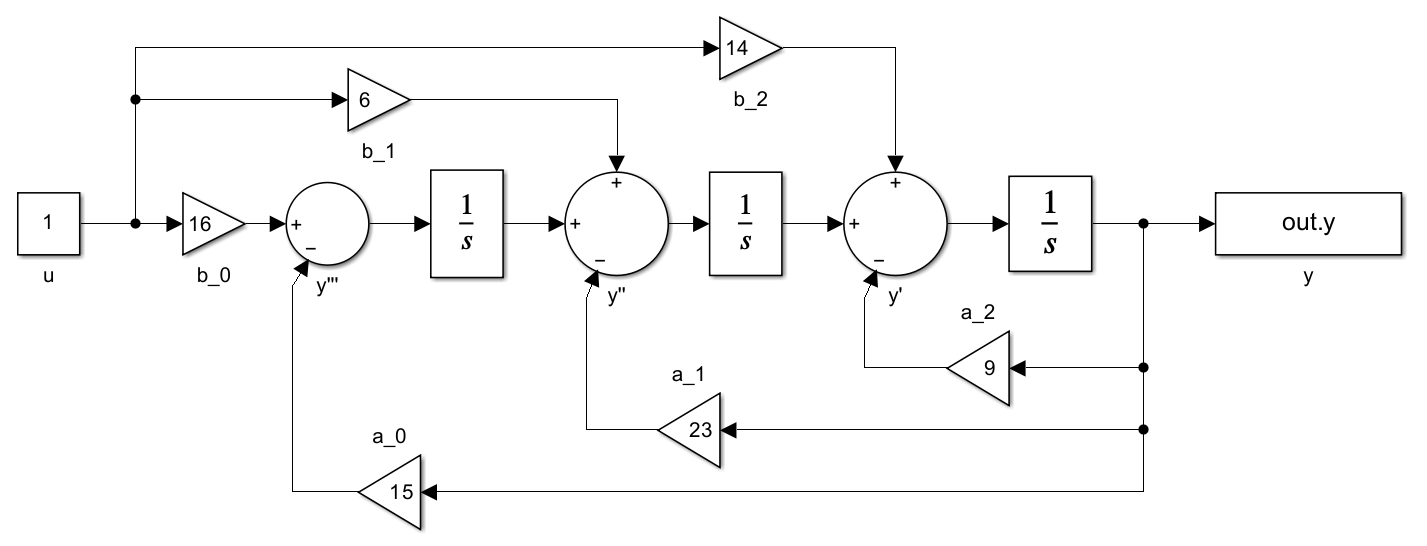
\includegraphics[width=1\linewidth]{pic/sch_1.png}}
\caption{Структурная схема первой системы.}
\end{figure}

\newpage
\subsection{Графики сигналов}

Выполним моделирование при входном воздействии вида $u(t)=1$ и нулевых начальных условиях $\ddot{y}(0)$, $\dot{y}(0)$, $y(0)$. Полученные графики выходных сигналов приведены на рисунке 2.

\begin{figure}[h]
\center{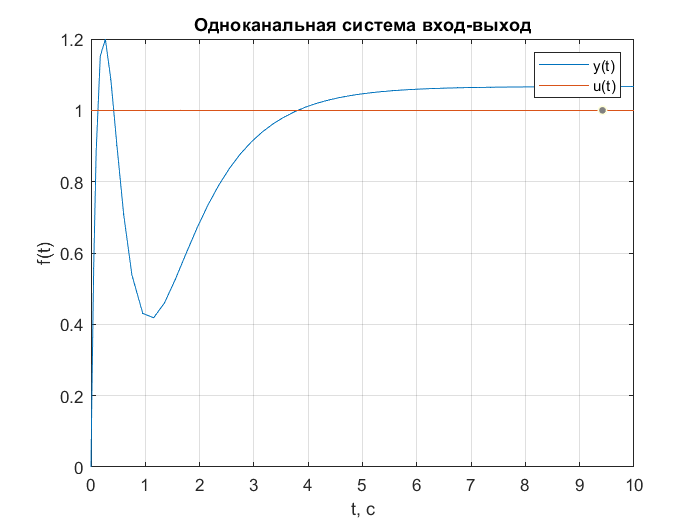
\includegraphics[width=1\linewidth]{pic/gr_1.png}}
\caption{Графики сигналов для одноканальной системы в форме вход-выход.}
\end{figure}

\newpage
\,
\newpage
\section{Задание. Переход от формы вход-выход к форме вход-состояние-выход}
\subsection{Математическая модель}
\subsubsection{Передаточная функция}
Для системы из 1 задания определим передаточную функцию $W(p)$.
\begin{equation}
\dddot{y} + 9\ddot{y} + 23 \dot{y} + 15 y = 14 \ddot{u} + 6 \dot{u} + 16 u
\end{equation}
Перепишем с применением оператора дифференцирования
\begin{multline}
p^3[y] + 9p^2[y] + 23 p[y] + 15 y = 14 p^2[u] + 6 p[u] + 16 u \Leftrightarrow \\
\Leftrightarrow \left( p^3 + 9p^2 + 23 p + 15 \right) [y] = \left( 14 p^2 + 6 p + 16 \right) [u] \Leftrightarrow \\
\Leftrightarrow  y = \frac{14 p^2 + 6 p + 16}{p^3 + 9p^2 + 23 p + 15} [u] + 0
\end{multline}
Получим передаточную функцию
\begin{equation}
W(p) = \frac{14 p^2 + 6 p + 16}{p^3 + 9p^2 + 23 p + 15}
\end{equation}


\subsubsection{Каноническая управляемая форма}

\begin{multline}
\begin{bmatrix}
\dot{x_1}\\
\dot{x_2}\\
\dot{x_3}
\end{bmatrix}
=
\begin{bmatrix}
0 & 1 & 0\\
0 & 0 & 1\\
-a_0 & -a_1 & -a_2
\end{bmatrix}
\begin{bmatrix}
x_1\\
x_2\\
x_3
\end{bmatrix}
+
\begin{bmatrix}
0\\
0\\
1
\end{bmatrix}
u \Leftrightarrow\\
\Leftrightarrow
\begin{bmatrix}
\dot{x_1}\\
\dot{x_2}\\
\dot{x_3}
\end{bmatrix}
=
\begin{bmatrix}
0 & 1 & 0\\
0 & 0 & 1\\
-15 & -23 & -9
\end{bmatrix}
\begin{bmatrix}
x_1\\
x_2\\
x_3
\end{bmatrix}
+
\begin{bmatrix}
0\\
0\\
1
\end{bmatrix}
u,\\
 y = 
\begin{bmatrix}
b_0 & b_1 & b_2
\end{bmatrix}
\begin{bmatrix}
x_1\\
x_2\\
x_3
\end{bmatrix}\Leftrightarrow
 y = 
\begin{bmatrix}
16 & 6 & 14
\end{bmatrix}
\begin{bmatrix}
x_1\\
x_2\\
x_3
\end{bmatrix}
\end{multline}

\subsubsection{Каноническая наблюдаемая форма}

\begin{multline}
\begin{bmatrix}
\dot{x_1}\\
\dot{x_2}\\
\dot{x_3}
\end{bmatrix}
=
\begin{bmatrix}
0 & 0 & -a_0\\
1 & 0 & -a_1\\
0 & 1 & -a_2
\end{bmatrix}
\begin{bmatrix}
x_1\\
x_2\\
x_3
\end{bmatrix}
+
\begin{bmatrix}
b_0\\
b_1\\
b_2
\end{bmatrix}
u \Leftrightarrow\\
 \Leftrightarrow
\begin{bmatrix}
\dot{x_1}\\
\dot{x_2}\\
\dot{x_3}
\end{bmatrix}
=
\begin{bmatrix}
0 & 0 & -15\\
1 & 0 & -23\\
0 & 1 & -9
\end{bmatrix}
\begin{bmatrix}
x_1\\
x_2\\
x_3
\end{bmatrix}
+
\begin{bmatrix}
16\\
6\\
14
\end{bmatrix}
u\\
y = 
\begin{bmatrix}
0 & 0 & 1
\end{bmatrix}
\begin{bmatrix}
x_1\\
x_2\\
x_3
\end{bmatrix} \Leftrightarrow\\
 \Leftrightarrow
y = 
\begin{bmatrix}
0 & 0 & 1
\end{bmatrix}
\begin{bmatrix}
x_1\\
x_2\\
x_3
\end{bmatrix} 
\end{multline}

\subsubsection{Каноническая диагональная форма}
\begin{multline}
\begin{bmatrix}
\dot{x_1}\\
\dot{x_2}\\
\dot{x_3}
\end{bmatrix}
=
\begin{bmatrix}
\lambda_1 & 0 & 0\\
0 & \lambda_2 & 0\\
0 & 0 & \lambda_3
\end{bmatrix}
\begin{bmatrix}
x_1\\
x_2\\
x_3
\end{bmatrix}
+
\begin{bmatrix}
\beta_1\\
\beta_2\\
\beta_3
\end{bmatrix}
u\\
y = 
\begin{bmatrix}
\gamma_1 & \gamma_2 & \gamma_3
\end{bmatrix}
\begin{bmatrix}
x_1\\
x_2\\
x_3
\end{bmatrix}\\
\end{multline}

Запишем передаточную функцию

\begin{equation}
W(p) = \frac{14 p^2 + 6 p + 16}{p^3 + 9 p^2 + 23 p + 15} 
\end{equation}

    Разложим знаменатель на произведение множителей. Заметим, что один из корней $p=-1$, после применения схемы Горнера останется квадратное уравнение, решение которого находится по теореме Виета

\begin{equation}
\left(p+1 \right) \left( p^2 + 8p + 15 \right) =  \left(p+1 \right) \left(p+3 \right) \left(p+5 \right)
\end{equation}

    Найдем разложение вида
\begin{multline}
      \frac{14 p^2 + 6 p + 16}{p^3 + 9 p^2 + 23 p + 15} = \frac{A}{p+1} + \frac{B}{p+3} + \frac{C}{p+5} =\\\\= \frac{A\left(p+3 \right) \left(p+5 \right) + B \left(p+1 \right) \left(p+5 \right) + C \left(p+3 \right) \left(p+1 \right)}{p^3 + 9 p^2 + 23 p + 15} = \\\\ =
      \frac{Ap^2+8Ap+15A+Bp^2+6Bp+5B+Cp^2+4Cp+3C}{p^3 + 9 p^2 + 23 p + 15} = \\\\ = \frac{\left( A + B + C\right) p^2 + \left( 8A + 6B + 4C\right)p  +15A+5B+3C}{p^3 + 9 p^2 + 23 p + 15} = \\\\ =
      \frac{3}{p+1} - \frac{31}{p+3} + \frac{42}{p+5}
\end{multline}
Теперь заметим, что

\begin{multline}
W(p) = \frac{\beta_1 \cdot \gamma_1}{p-\lambda_1} + \frac{\beta_2 \cdot \gamma_2}{p-\lambda_2} + \frac{\beta_3 \cdot \gamma_3}{p-\lambda_3} = \frac{3}{p+1} - \frac{31}{p+3} + \frac{42}{p+5} =\\
= \frac{3 \cdot 1}{p+1} + \frac{31 \cdot (-1)}{p+3} + \frac{6 \cdot 7}{p+5}
\end{multline}

Наконец запишем систему в канонической диагональной форме.
\begin{multline}
\begin{bmatrix}
\dot{x_1}\\
\dot{x_2}\\
\dot{x_3}
\end{bmatrix}
=
\begin{bmatrix}
-1 & 0 & 0\\
0 & -3 & 0\\
0 & 0 & -5
\end{bmatrix}
\begin{bmatrix}
x_1\\
x_2\\
x_3
\end{bmatrix}
+
\begin{bmatrix}
3\\
31\\
6
\end{bmatrix}
u\\
y = 
\begin{bmatrix}
1 & -1 & 7
\end{bmatrix}
\begin{bmatrix}
x_1\\
x_2\\
x_3
\end{bmatrix}\\
\end{multline}

\subsection{Структурные схемы системы для представления В-С-В и соответствующие графики}

\subsubsection{Передаточная функция}

\begin{figure}[h]
\center{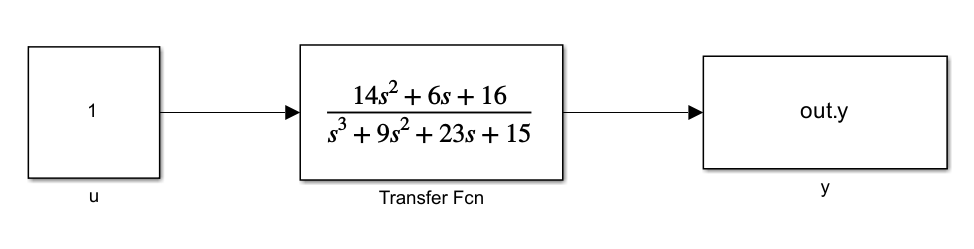
\includegraphics[width=1\linewidth]{pic/sch_2_1.png}}
\caption{Структурная схема с использованием передаточной функции.}
\end{figure}

\begin{figure}[h]
\center{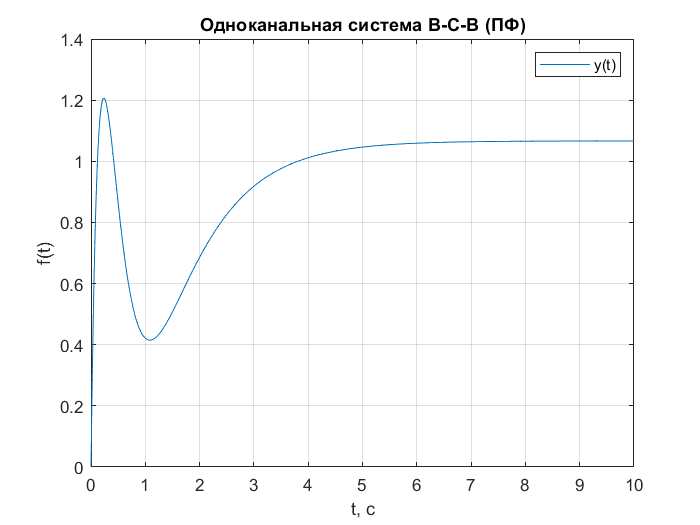
\includegraphics[width=0.8\linewidth]{pic/gr_2_1.png}}
\caption{График системы с использованием передаточной функции.}
\end{figure}

\subsubsection{Каноническая управляемая форма}


\subsubsection{Каноническая наблюдаемая форма}


\subsubsection{Каноническая диагональная форма}


\end{document}













